\chapter{Analisi Concorrenza e Distribuzione}

La modellazione di un sistema ferroviario presenta diverse problematiche relative alla concorrenza e alla distribuzione. Di seguito verranno presentate le più rilevanti.

\section{Ingresso in un Segmento da parte di un Treno}\label{ingresso_segmento}

\begin{figure}[htbp]
	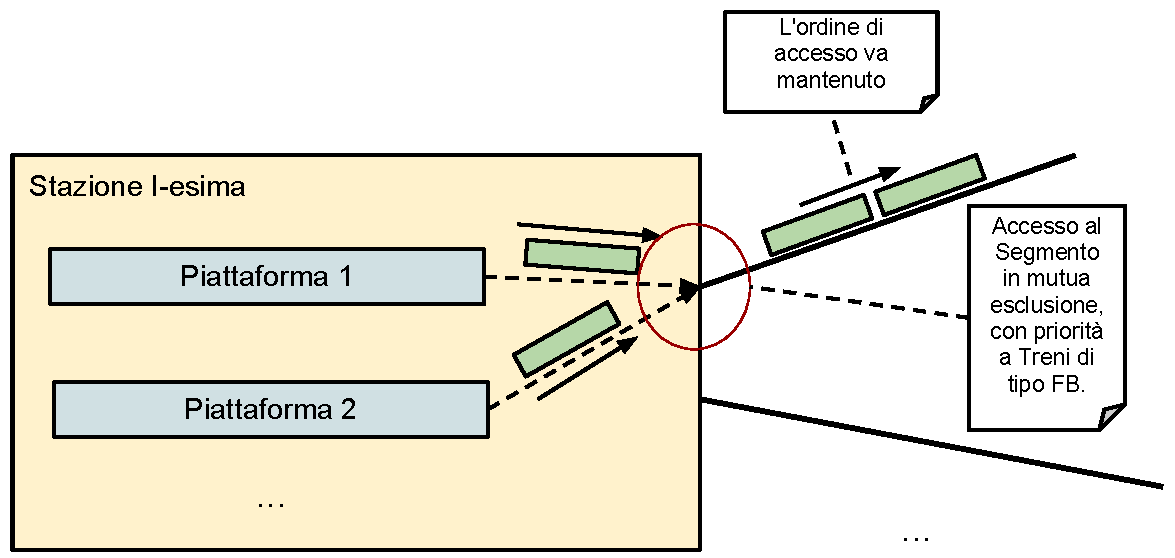
\includegraphics[width=\textwidth,keepaspectratio]{imgs/ingresso_segmento.pdf}
	\caption{\footnotesize{Accesso ad un Segmento da Parte di uno o più Treni.}}
\end{figure}

L'accesso ad un segmento di collegamento tra due stazioni da parte di un Treno, è inerentemente concorrente. Tale azione presenta infatti i seguenti requisiti:
	\begin{itemize}
		\item L'ingresso presso un Segmento deve avvenire in \ii{mutua esclusione}; è infatti impossibile che due o più entità Treno accedano ad uno stesso Segmento contemporaneamente.
		\item Più Treni possono circolare su un Segmento contemporaneamente. Questo comporta:
			\begin{itemize}
				\item il mantenimento di un ordine di ingresso al Segmento;
				\item la regolazione della velocità di transito di ciascun Treno in base alla velocità di quelli che lo precedono;
				\item l'impossibilità di un Treno di accedere ad un Segmento qualora vi siano altri Treni che lo percorrono in senso opposto.
			\end{itemize}
		\item Dev'essere data precedenza d'accesso al Segmento, ai Treni di tipo \ttt{FB}.
	\end{itemize}


\section{Uscita da un Segmento e accesso alla Stazione}

\begin{figure}[htbp]
	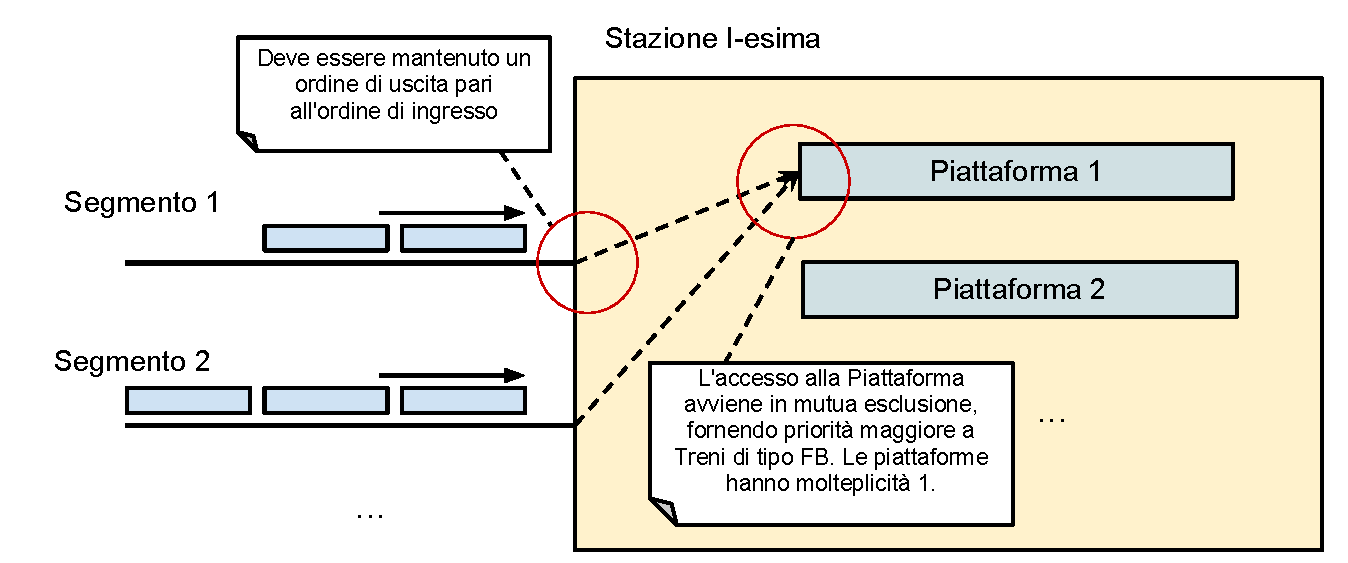
\includegraphics[width=\textwidth,keepaspectratio]{imgs/Ingresso_Stazione.pdf}
	\caption{\footnotesize{Uscita da un Segmento e accesso ad una Piattaforma di uno o più Treni.}}
\end{figure}

Il problema introdotto in sezione \ref{ingresso_segmento}, vincola i requisiti che dovranno essere soddisfatti relativamente all'uscita da un Segmento e conseguente accesso alla Stazione successiva. Per queanto riguarda l'uscita dal Segmento avremo quindi i seguenti requisiti:
	\begin{itemize}
		\item L'ordine di ingresso al Segmento dev'essere mantenuto all'uscita. 
		\item L'ordine di uscita da un Segmento dev'essere mantenuto nell'accesso alla stazione successiva da parte dei Treni in transito.
	\end{itemize}

L'ingresso in una Stazione, permette ad un Treno di occupare una della Piattaforme disponibili e, dato che da specifica una stazione può essere raggiunta da più Segmenti, tale azione sarà svolta in modo concorrente tra i treni in uscita dai vari Segmenti, secondo i seguenti vincoli:
	\begin{itemize}
		\item I Treni di tipo \ttt{FB} avranno priorità maggiore nell'occupare una Piattaforma.
		\item Ciascuna Piattaforma è acceduta in mutua esclusione, e può essere occupata da un solo Treno alla volta.  
	\end{itemize}

Questo significa che l'accesso ad una Piattaforma sarà ordinato, per tutti i Treni provenienti dallo stesso Segmento, in base all'ordine di uscita da quest'ultimo, e concorrente tra Treni provenienti da Segmenti diversi. 

\section{Acquisto di un Biglietto da parte di un Viaggiatore}

Ciascun Viaggiatore deve acquistare un biglietto prima di poter usufruire dei servizi ferroviari. Per fare ciò, all'interno ogni stazione vi è una Biglietteria presso la quale l'acquisto può essere effettuato. Un biglietto sarà composto da una serie di Tappe, ciascuna relativa ad un tratto del percorso da portare a termine con uno specifico Treno, sia Regionale che FB. 
L'assegnazione di un Biglietto ad un Viaggiatore è semplice se il suo percorso prevede solo l'utilizzo di Treni Regionli, mentre è più complesso se vi sono tappe da raggiungere con Treni FB, i cui biglietti vengono erogari se e soltanto se vi è ancora posto all'interno del treno.
\'E quindi necessario prevedere l'esistenza di una \ii{biglietteria centrale} che mantenga le prenotazioni dei Treni di tipo FB. Si ricavano quindi i seguenti requisiti:
	\begin{itemize}
		\item La biglietteria centrale va acceduta in mutua esclusione, in modo da evitare prenotazioni inconsistenti di Biglietti.
		\item L'erogazione di biglietti può fallire in caso non vi siano posti per percorrere alcune tappe; il sistema deve reagire di conseguenza.
	\end{itemize}

